\section{从一道简单而基础的数学题出发}
\subsection{平面中求面积}
\subsubsection{引题}

  \prob 如图\ref{pro1},在平面直角坐标系中
  ,已知$A(2,3)$,$B(1,5)$,求$S_{\triangle ABO}$.

  \sol由$O(0,0),B(1,5)$可知
  $$OB:5x-y=0,$$
  $$\abs{OB}=\sqrt{(1-0)^2+(5-0)^2}=\sqrt{26},$$
  又$A(2,3)$,则$OB$边上高
  $$h=\frac{\abs{10-3}}{\sqrt{5^2+1^2}}=\frac{7}{\sqrt{26}},$$
  故
  $$S_{\triangle ABO}=\frac{1}{2}\abs{OB}\times h=\frac{7}{2}.$$
\solend

\sol如图\ref{pro2},用矩形(粗线部分)减去三个小三角形
\begin{eqnarray}
S_{\triangle OAB}
&=&S_{OCDB}-S_{\triangle OCB}-
S_{\triangle OEA}-S_{\triangle ABD} \nonumber\\
&=&10-\frac{5}{2}-3-1\nonumber\\
&=&\frac{7}{2}.\nonumber
\end{eqnarray}
\solend

\begin{figure}
  \centering
  % Requires \usepackage{graphicx}
  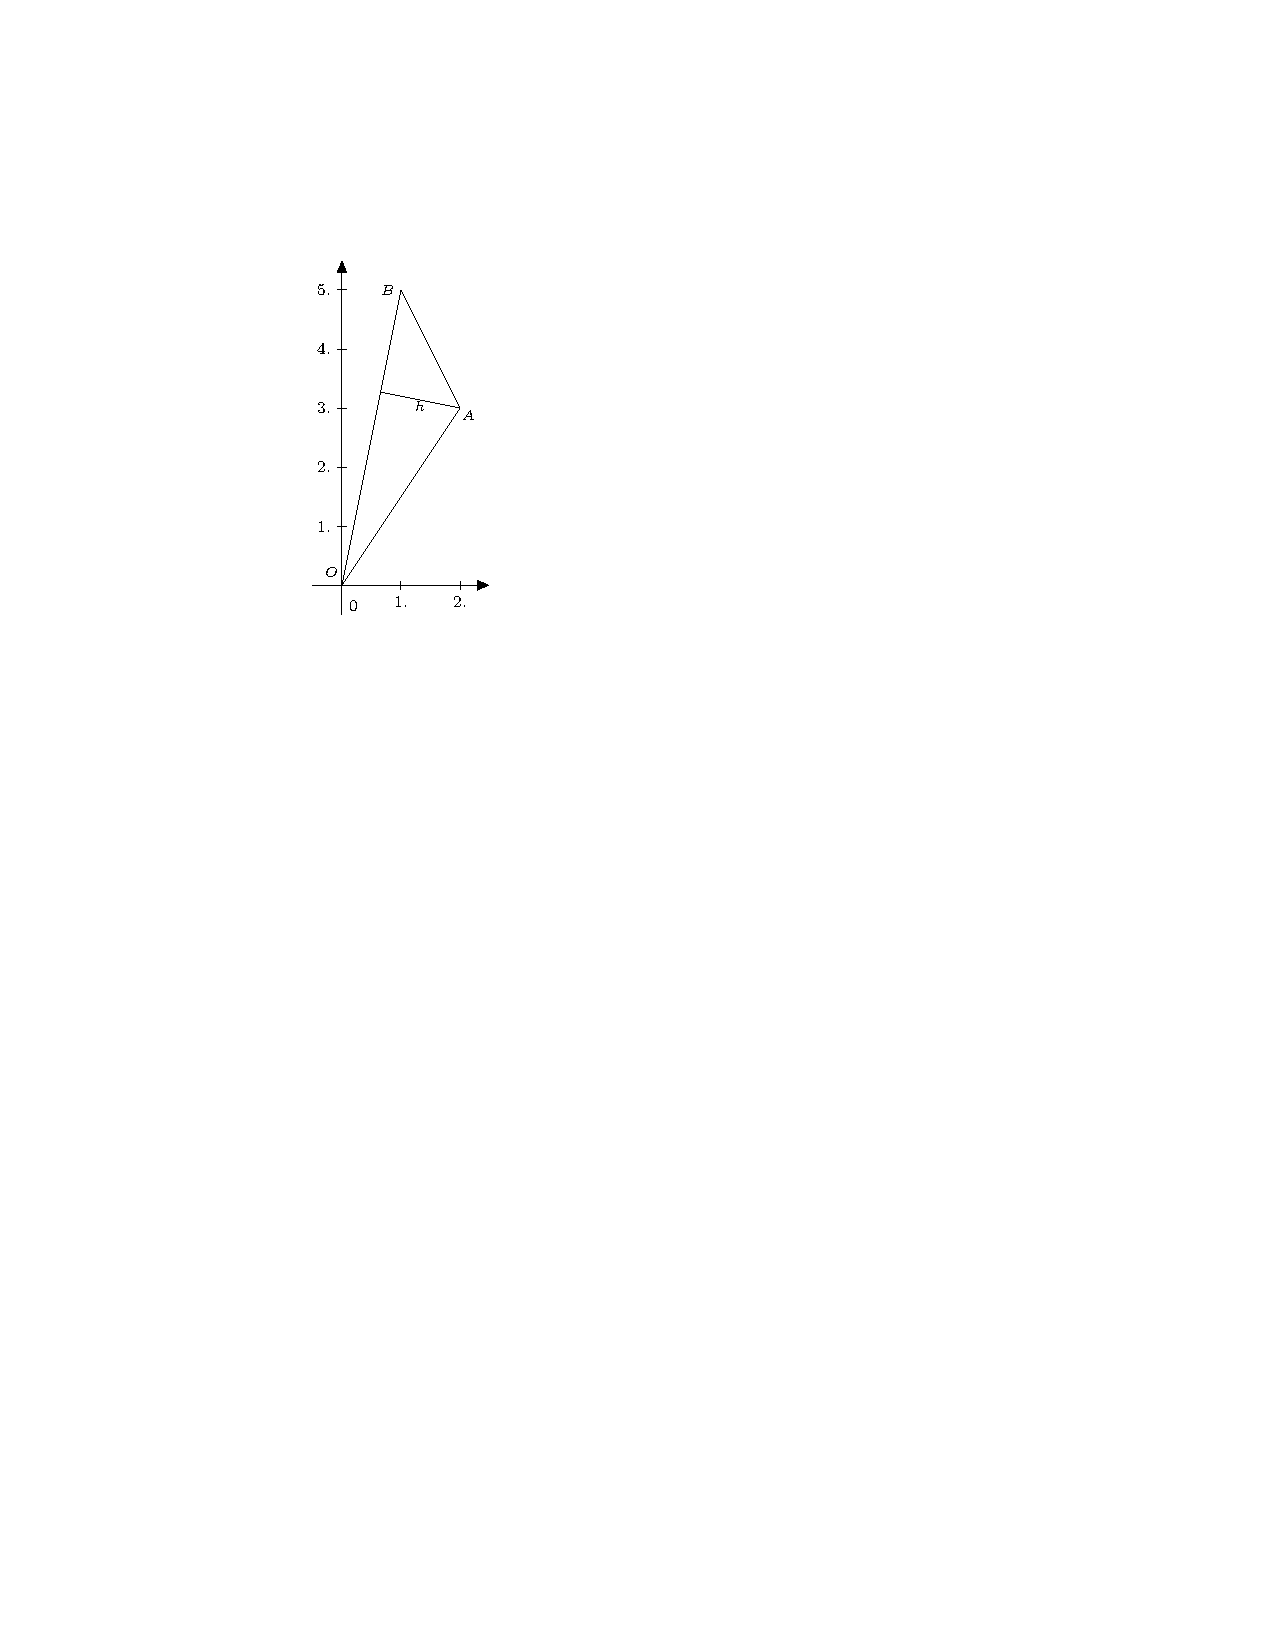
\includegraphics[width=3cm]{pic//1//1.pdf}\\
  \caption{一道简单而基础的数学题}\label{pro1}
\end{figure}

\begin{figure}
  \centering
  % Requires \usepackage{graphicx}
  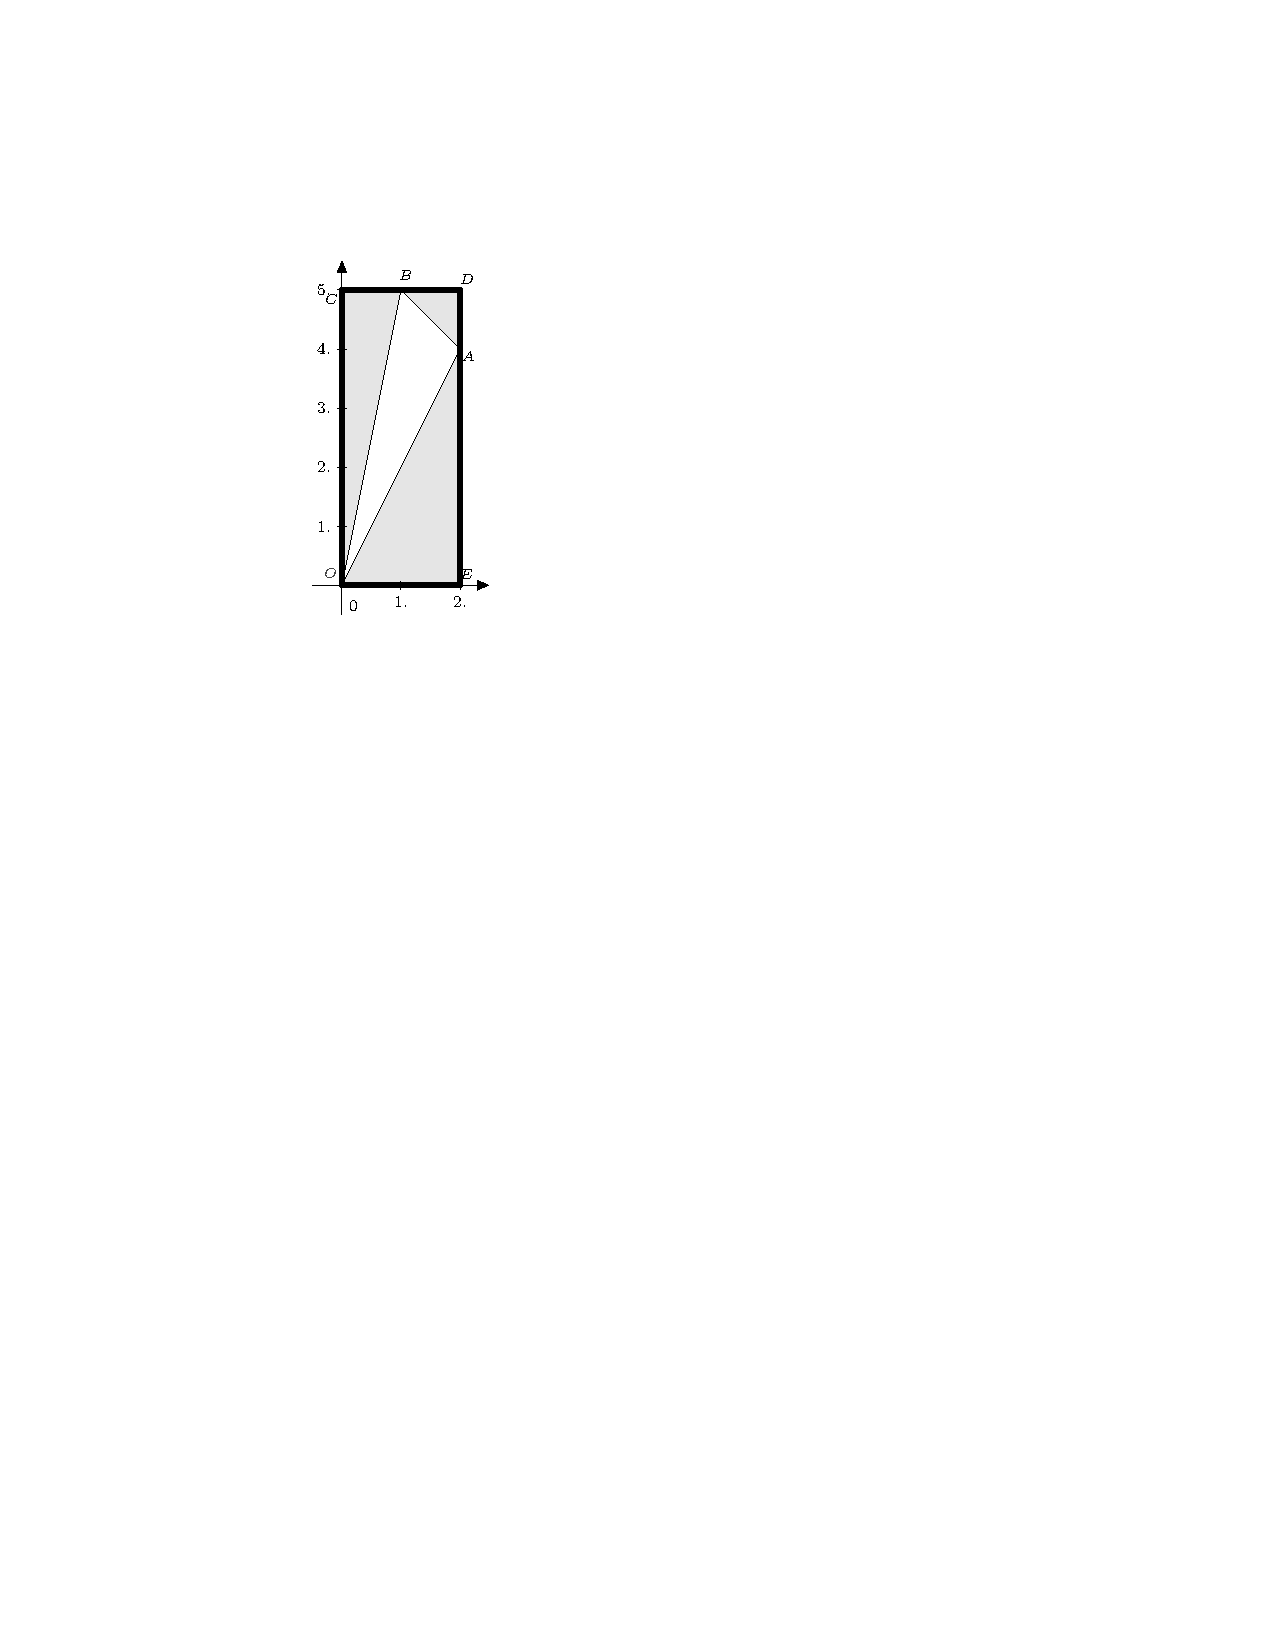
\includegraphics[width=3cm]{pic//2//2.pdf}\\
  \caption{方若愚的解法}\label{pro2}
\end{figure}

\subsubsection{引题的一般情况}
考虑引题的一般情况:

\prob 已知两点$A(x_1,y_1),B(x_2,y_2)$,求$\dps S_{\triangle OAB}$.

\sol用上面提到的两种方法均可解答,易知
$$
S_{\triangle OAB}=\frac{1}{2}\abs{x_1y_2-x_2y_1}
=\abs{\abs{\begin{array}{cc}
  x_1&y_1\\
  x_2&y_2\\ 
\end{array}}}.
$$
\solend

\prob 已知三点$A,B,C$,坐标分别为$(x_i,y_i)(i=1,2,3)$,求$S_{\triangle ABC}$.

\sol由$A(x_1,y_1),B(x_2,y_2)$可知
$$AB:(y_1-y_2)x-(x_1-x_2)y+(x_1y_2-x_2y_1)=0,$$
$$\abs{AB}=\sqrt{(x_1-x_2)^2+(y_1-y_2)^2},$$
又$C(x_3,y_3)$,则$AB$边上高
$$h=\frac{\abs{(y_1-y_2)x_3-(x_1-x_2)y_3}}
{\sqrt{(y_1-y_2)^2+(x_1-x_2)^2}},$$
故
\begin{eqnarray}
  S_{\triangle ABC}&=&\frac{1}{2}\cdot h \abs{AB}\nonumber\\
  &=&\frac{1}{2}\cdot \frac{\abs{(y_1-y_2)x_3-(x_1-x_2)y_3+(x_1y_2-x_2y_1)}}
    {\sqrt{(y_1-y_2)^2+(x_1-x_2)^2}}
    \sqrt{(x_1-x_2)^2+(y_1-y_2)^2}\nonumber\\
  &=&\frac{1}{2}\abs{(y_1-y_2)x_3-(x_1-x_2)y_3+(x_1y_2-x_2y_1)}\nonumber\\
  &=&\frac{1}{2}\abs{x_1y_2-x_1y_3+x_2y_3-x_2y_1+x_3y_1-x_3y_2}\nonumber
\end{eqnarray}
\solend

\sol 将三角形做平移变换,将
$$ A(x_1,y_1),B(x_2,y_2),C(x_3,z_3)$$
平移为
$$A(0,0),B(x_2-x_1,y_2-y_1),C(x_3-x_1,y_3-y_1),$$
利用上一问的结论,有
$$S_{\triangle ABC}=
\abs{\abs{\begin{array}{cc}
  x_2-x_1&y_2-y_1\\
  x_3-x_1&y_3-y_1\\ 
\end{array}}}.
$$
\solend

本着对称轮换、简单优美的原则,我们有$$S_{\triangle ABC}=
\frac{1}{2}\left|\left|\begin{array}{ccc}
    1 & 1 & 1 \\
    x_1 & x_2 & x_3 \\  
    y_1 & y_2 & y_3 
  \end{array}\right|\right|.
%  =
%\frac{1}{2}\left|\left|\begin{array}{cc}
%    x_2-x_1 & y_2-y_1 \\
%    x_3-x_1 & x_3-y_1 
%  \end{array}\right|\right|
%  =\frac{1}{2}\abs{\vv{AB}\times\vv{AC}}
$$

\subsection{空间中求面积}

\prob 在空间直角坐标系中,已知三点$A,B,C,
\textrm{坐标为}(x_i,y_i,z_i)(i=1,2,3)$,
求$S_{\triangle ABC}$(以下简写为$S$).

我们先来看下面一种解法
\footnote{该解法由文子龙提供,他在研究这道题目时曾说:
``简单嘛,直接用三角形面积公式爆算''}.

\newcommand{\aaa}{\sqrt{(x_2-x_3)^2+(y_2-y_3)^2+(z_2-z_3)^2}}
\newcommand{\bbb}{\sqrt{(x_3-x_1)^2+(y_3-y_1)^2+(z_3-z_1)^2}}
\newcommand{\ccc}{\sqrt{(x_1-x_2)^2+(y_1-y_2)^2+(z_1-z_2)^2}}
\newcommand{\qqq}{q}

\sol
%q=\frac{1}{2}(a+b+c)\\
%=\frac{1}{2}(\aaa+)
%\textrm{则}\\
%S
%=\sqrt{q(q-a)(q-b)(q-c)}\\
%=\sqrt{\qqq(\qqq-\aaa)(\qqq-\bbb)(\qqq-\ccc)}
% 
令
\begin{eqnarray}
a&=&\aaa, \nonumber\\
b&=&\bbb, \nonumber\\
c&=&\ccc, \nonumber\\
q&=&\frac{1}{2}(a+b+c) \nonumber\\
 &=& \frac{1}{2}(\aaa \nonumber\\
 && +\bbb \nonumber\\
 && +\ccc \nonumber),
\end{eqnarray}
则$$S=\sqrt{T},$$
其中
\begin{eqnarray}
  T&=&q(q-a)(q-b)(q-c) \nonumber \\  
  &=&\cdots(\textrm{代入}q,a,b,c) \nonumber \\
  &=&\cdots(\textrm{化简}) \nonumber \\
  &=&\cdots \nonumber 
\end{eqnarray}
\solend

上面的方法计算量巨大,不推荐采纳.

\begin{figure}
  \centering
  % Requires \usepackage{graphicx}
  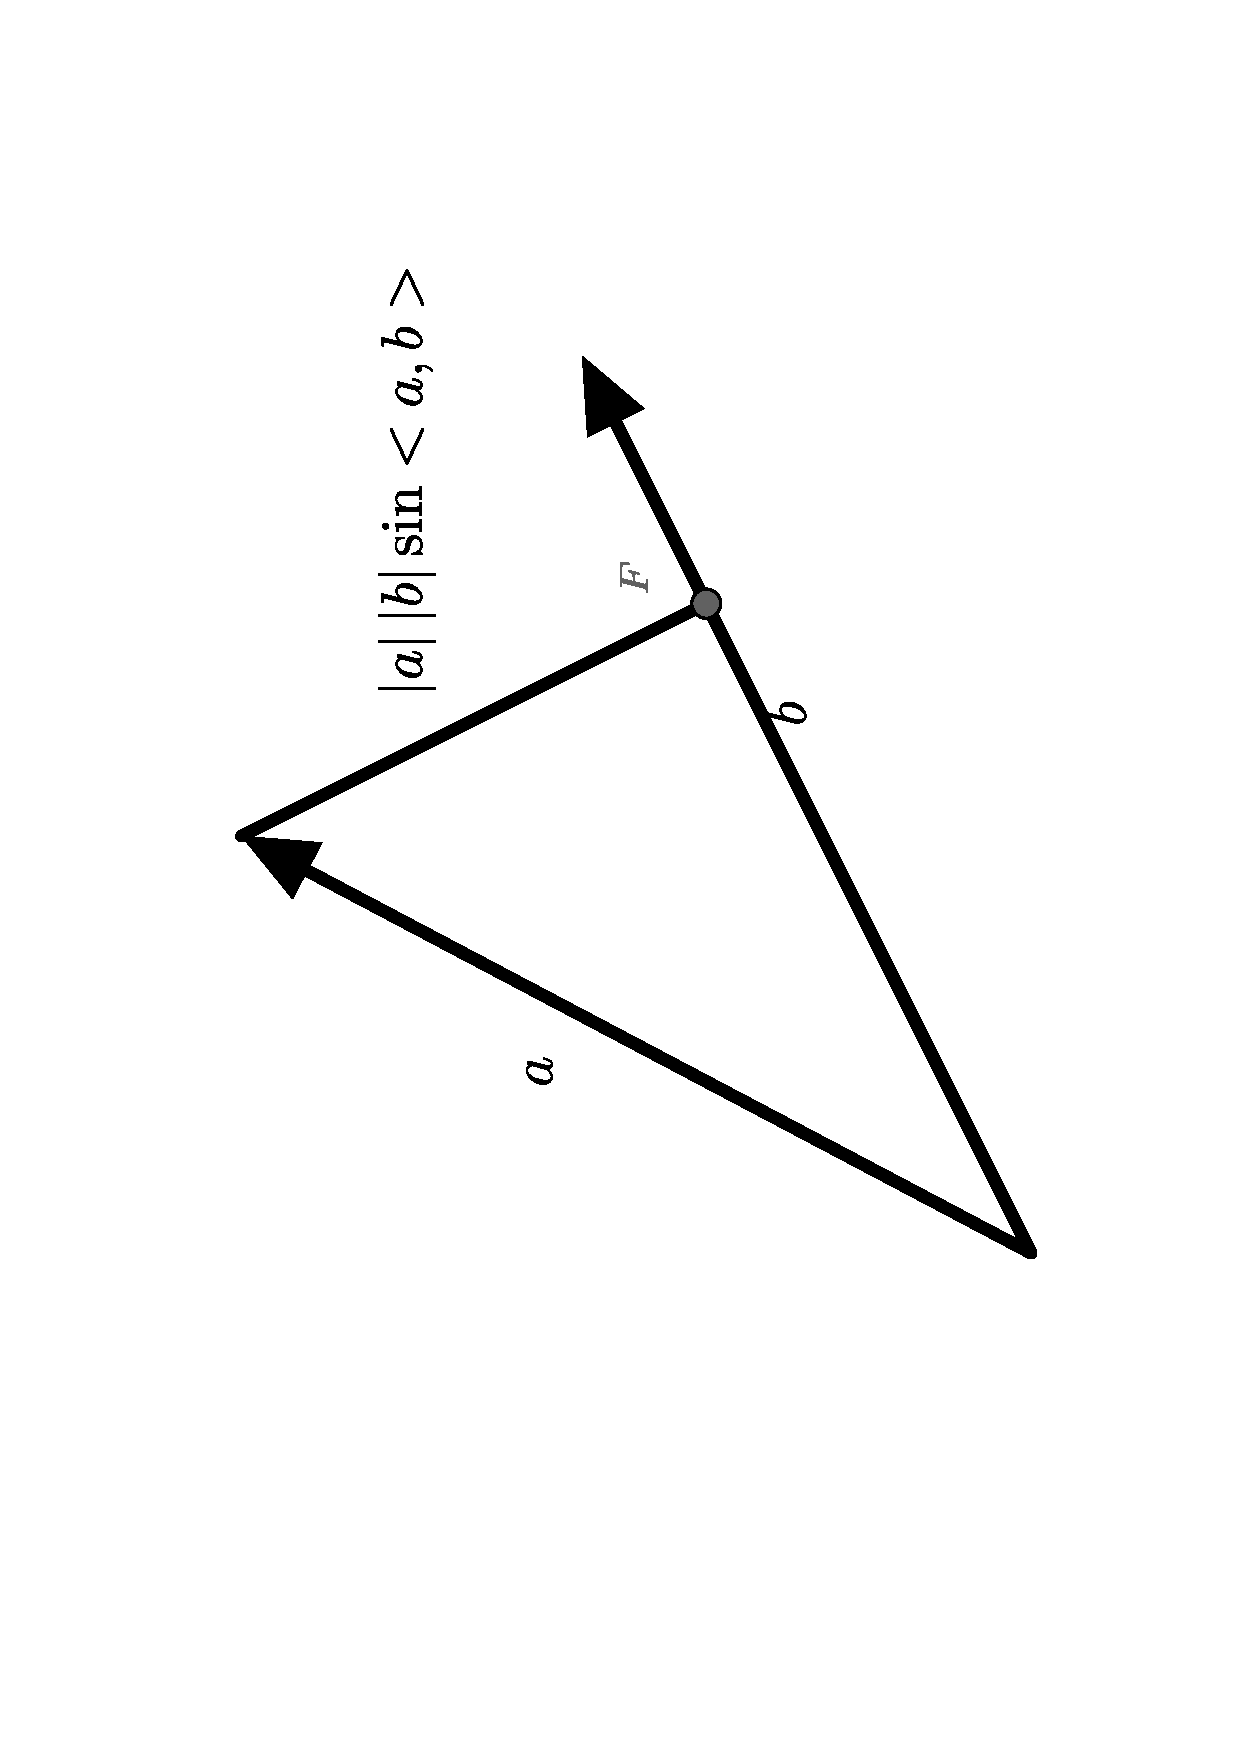
\includegraphics[width=6cm,angle=270]{pic//3//33.pdf}\\
  \caption{向量积的模}\label{pro3}
\end{figure}

\sol 如图\ref{pro3}($F$是垂足),
注意到向量积的(部分)定义式
$$\abs{\bm{a}\times\bm{b}}=\abs{\bm{a}}\abs{\bm{b}}\sin<a,b>$$
本身就表示以$\bm{a},\bm{b}$为邻边的平行四边形的面积.
建立标准单位向量\footnote{
  未作特别说明,分别以$\bm{i},\bm{j},\bm{k}$记$x$轴,$y$轴,$z$
  轴上与该轴正向同方向的单位向量
  }
  $\bm{i},\bm{j},\bm{k}$, 将向量用坐标表示
\begin{eqnarray}
\vv{AB}&=&(x_2-x_1,y_2-y_1,z_2-z_1),\nonumber\\
\vv{AC}&=&(x_3-x_1,y_3-y_1,z_3-z_1),\nonumber
\end{eqnarray}
则
\begin{eqnarray}
  S&=&\frac{1}{2}\abs{\vv{AB}\times\vv{AC}}\nonumber\\
  &=&\frac{1}{2}\abs
  {(x_2-x_1,y_2-y_1,z_2-z_1)\times
  (x_3-x_1,y_3-y_1,z_3-z_1)}\nonumber\\
  &=&\frac{1}{2}\left|\left|
  \begin{array}{ccc}
    \bm{i} & \bm{j} & \bm{k} \\
    x_2-x_1 & y_2-y_1  & z_2-z_1 \\
    x_3-x_1 &y_3-y_1  & z_3-z_1 \\
  \end{array}
  \right|\right|\nonumber\\
  &=&\frac{1}{2}\left|\left|
  \begin{array}{cccc}
    \bm{i}&\bm{j}&\bm{k}&0\\
    x_1&y_1&z_1&1\\
    x_2&y_2 &z_2&1\\
    x_3&y_3&z_3&1\\
  \end{array}
  \right|\right|\nonumber\\
  &=&\frac{1}{2}\sqrt
  {
    {T_1}^2+
    {T_2}^2+
    {T_3}^2
  }\nonumber.
\end{eqnarray}
其中
$$
T_1=\left|\begin{array}{ccc}
          y_1&z_1&1\\
          y_2&z_2&1\\
          y_3&z_3&1
          \end{array}\right|,
T_2=\left|\begin{array}{ccc}
  z_1&x_1&1\\
  z_2&x_2&1\\
  z_3&x_3&1
  \end{array}\right|,
T_3=\left|\begin{array}{ccc}
  x_1&y_1&1\\
  x_2&y_2&1\\
  x_3&y_3&1
  \end{array}\right|.
$$
\solend

注意,在上面的解答中出现的
$$
\left|
  \begin{array}{cccc}
    \bm{i}&\bm{j}&\bm{k}&0\\
    x_1&y_1&z_1&1\\
    x_2&y_2 &z_2&1\\
    x_3&y_3&z_3&1\\
  \end{array}
  \right|
$$
(显然地)表示平面$ABC$的法向量.

\prob 在空间直角坐标系中,已知两点$A,B
\textrm{坐标为}(x_i,y_i,z_i)(i=1,2)$,
求$S_{\triangle OAB}$(以下简写为$S$).

\sol 与上一道例题类似.这里直接给出结果
$$S=\frac{1}{2}\sqrt{T_1^2+T_2^2+T_3^2},$$
其中
$$
T_1=\left|\begin{array}{cc}
  y_1&z_1\\
  y_2&z_2
  \end{array}\right|
  ,
T_2=\left|\begin{array}{cc}
  z_1&x_1\\
  z_2&x_2
  \end{array}\right|
  ,
T_3=\left|\begin{array}{cc}
  x_1&y_1\\
  x_2&y_2
  \end{array}\right|
  .
$$ 
\solend

\subsection{空间中求体积}

\prob 在空间直角坐标系中,已知三点$A,B,C,
\textrm{坐标为}(x_i,y_i,z_i)(i=1,2,3)$,
求$V_{\textrm{三棱锥}OABC}$(以下简写为$V$).

\sol 首先我们有
\begin{eqnarray}
V&=&\frac{1}{3}S\cdot h\nonumber,
\end{eqnarray}
而
\begin{eqnarray}
S&=&\frac{1}{2}\left |\vv{OA}\times \vv{OB} \right|\nonumber,\\
h&=&\left|\vv{OC} \right| \cdot \cos<\textrm{面OAB,直线OC}>\nonumber,
\end{eqnarray}
注意到
\begin{eqnarray}
\cos<\textrm{面OAB,直线OC}>=\left|\cos<\vv{OA}\times \vv{OB},\vv{OC}>\right|\nonumber,
\end{eqnarray}
故
\begin{eqnarray}
V&=&\frac{1}{6}\abs{\vv{OA}\times\vv{OB}}\abs{\vv{OC}}
    \cos<\vv{OA}\times \vv{OB},\vv{OC}>\nonumber\\
    \label{mixedProduct}
 &=&\frac{1}{6}\left|\left(\vv{OA}\times
 \vv{OB}\right)\cdot\vv{OC} \right|.
\end{eqnarray}
在式(\ref{mixedProduct})中同时用到了向量的数量积和向量积,
$(\bm{a}\times\bm{b})\cdot\bm{c}$ 
 称为(向量)$\bm{a},\bm{b},\bm{c}$的
 混合积,是一个数.又已知
 $$
 \vv{OA}\times\vv{OB}=
 \left(
 \left|
   \begin{array}{cc}
     y_1&z_1\\
     y_2&z_2\\
   \end{array}
 \right|
 ,
 \left|
   \begin{array}{cc}
     z_1&x_1\\
     z_2&x_2\\
   \end{array}
 \right|
 ,
 \left|
   \begin{array}{cc}
     x_1&y_1\\
     x_2&y_2\\
   \end{array}
 \right|
 \right),
 $$
 所以
 \begin{eqnarray}
  \left(\vv{OA}\times\vv{OB}\right)\cdot\vv{OC}
  &=&
  \left|
    \begin{array}{cc}
      y_1&z_1\\
      y_2&z_2\\
    \end{array}
  \right|
  x_3+
  \left|
    \begin{array}{cc}
      z_1&x_1\\
      z_2&x_2\\
    \end{array}
  \right|
  y_3+
  \left|
    \begin{array}{cc}
      x_1&y_1\\
      x_2&y_2\\
    \end{array}
  \right|
  z_3\nonumber\\
  &=&
  \left|
    \begin{array}{ccc}
      x_1&y_1&z_1\\
      x_2&y_2&z_2\\
      x_3&y_3&z_3
    \end{array}
  \right|\nonumber,
 \end{eqnarray}
 则
 $$
 V=\frac{1}{6}
 \left|\left|
    \begin{array}{ccc}
      x_1&y_1&z_1\\
      x_2&y_2&z_2\\
      x_3&y_3&z_3
    \end{array}
  \right|\right|.
 $$
 \solend

 \prob 在空间直角坐标系中,已知四点$A,B,C,D
 \textrm{坐标为}(x_i,y_i,z_i)(i=1,2,3,4)$,
 求$V_{\textrm{三棱锥}ABCD}$(以下简写为$V$).

\sol 这里直接给出答案
$$
V=\frac{1}{6}\cdot
\left|
    \begin{array}{cccc}
      x_1&y_1&z_1&1\\
      x_2&y_2&z_2&1\\
      x_3&y_3&z_3&1\\
      x_4&y_4&z_4&1\\
    \end{array}
  \right|.
$$
\solend
